\chapter{Implementacija i korisničko sučelje}


\section{Korištene tehnologije i alati}

\normalfont Aplikacija je napisana kao Maven Projekt. Maven je alat korišten primarno za java projekte zbog lakšeg i preglednijeg upravljanja projektom. Backend dio aplikacije pisan je u jeziku Java i korišten je radni okvir Spring Boot dok je frontend pisan pomoću Bootstrap radnog okvira. Spring Boot omogućava brži i efikasniji pristup izgradnje Spring aplikacije i Spring web aplikacije. Pruža široki spektar opcija te olakšava posao korisniku tako da se ne treba brinuti o raznim implementacijskim detaljima.

\normalfont\noindent Za razvojno okruženje korišten je IntelliJ Idea Ultimate. IntelliJ je razvojno okruženje koje je razvila tvrtka JetBrains i služi za razvijanje i pisanje računalnog softvera u programskom jeziku javi.

\normalfont\noindent Kao web poslužitelj uzet je Apache Tomcat, a za rad s bazom podataka koristio se H2 Database. Apache Tomcat je open source web poslužitelj koji implementira nekoliko Java EE specifikacija. Također je korišten iz razloga što je direktno ugrađen u Spring Boot framework. H2 je open source baza podataka koja omogućuje korištenje tako da podaci ne ostaju na disku.

\normalfont\noindent Komunikacija u timu realizirana je pomoću aplikacije Slack i aplikacije WhatsApp. Sustav za upravljanje kodom korišten je Git a repozitorij projekta je dostupan na web platformi GitLab. 

\bigskip

\noindent\url{https://maven.apache.org/}\\
\url{https://spring.io/projects/spring-boot}\\
\url{https://www.oracle.com/java/technologies/}\\
\url{https://getbootstrap.com/ }\\
\url{http://tomcat.apache.org/}\\
\url{https://www.h2database.com/html/main.html}\\
\url{https://slack.com/intl/en-hr/}\\
\url{https://web.whatsapp.com/}

\eject 


\section{Ispitivanje programskog rješenja}


\subsection{Ispitivanje komponenti}

\bigskip

\normalfont Testovi za ispitivanje pojedinih komponenti backend dijela aplikacije izvršeni su pomoću JUnit alata. Cilj ovih testova je provjera ispravnosti rada u programu za osnovne funkcionalnosti sustava, te za lakše otkrivanje pogrešaka kod nekih nespecifičnih slučajeva. 

\normalcolor\noindent Jedan od testiranih komponenti je dodavanje događaja od strane organizatora. Sustav svaki pokušaj unosa događaja provjerava pomoću validatora. Validator metodom „validate“ prima EventForm objekt koji je ispunjen informacijama unesenih od strane organizatora i BindingResults pomoću kojeg vraća greške. Na slici \ref{fig:ispitivanjeunosadogadaja} prikazano je dva testa, prvi simulira ispravan unos informacija za događaj a drugi neispravan tako što fali ime i opis događaja.


\begin{figure}[H]
	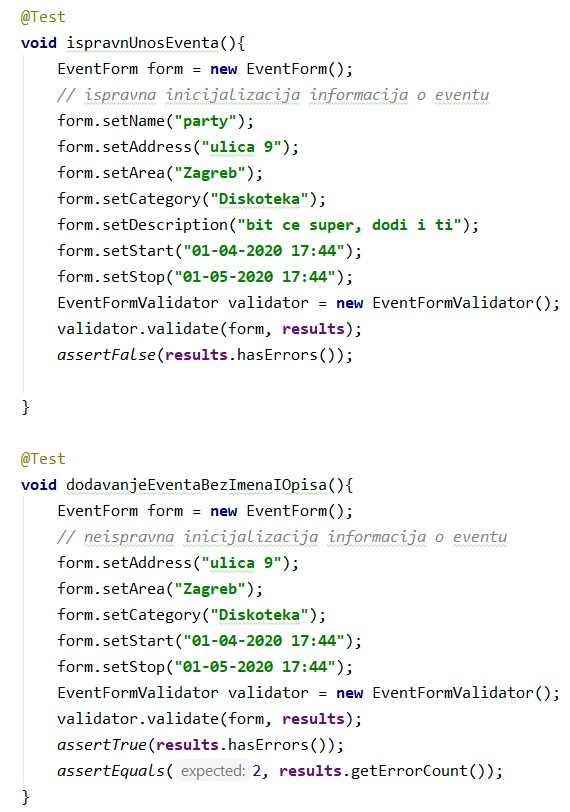
\includegraphics[scale=0.6]{slike/ispitivanje_unosa_dogadaja.jpeg}
	\centering
	\caption{Ispitivanje ispravnog i neispravnog unosa događaja}
	\label{fig:ispitivanjeunosadogadaja}
\end{figure}

\normalfont Osim ne upisanih informacija o događaju, sustav provjerava jesu li te informacije smislene. Npr na slici \ref{fig:pogresanunosdatuma} prikazana su dva testa kod kojih su krivo uneseni datumi početka i kraja događaja. Prvi test provjerava baca li validator pogrešku ako je uneseni datum završetka događaja prije datuma početka. Drugi test provjerava također jeli validator bacio pogrešku kada je datum početka događaja prije današnjeg datuma.

\begin{figure}[H]
	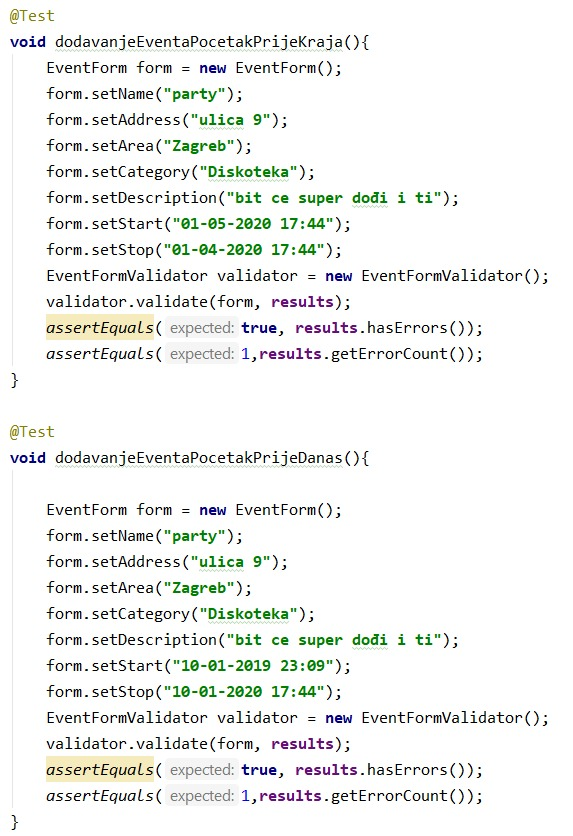
\includegraphics[scale=0.6]{slike/pogresan_unos_datuma.jpeg}
	\centering
	\caption{Ispitivanje pogrešnog unosa datuma}
	\label{fig:pogresanunosdatuma}
\end{figure}

\normalfont Uz ove već navedene informacije, korisnik također mora odabrati kategoriju i mjesto događaja pomoću „drop down“ liste. Ako je korisnik zaboravio odabrati primjerice kategoriju, u EventForm objekt će biti zapisano „Izaberi kategoriju“. Validator to provjerava i javlja grešku. Zadnji test na slici \ref{fig:kategorijaimjestodogadaja} ispituje jeli korisnik izabrao kategoriju i mjesto događaja. Uovom slučaju se simulira kao da korisnik nije naveo ni jedno ni drugo tako da validator baca dvije pogreške što se može iščitati iz BindingResults objekta.

\begin{figure}[H]
	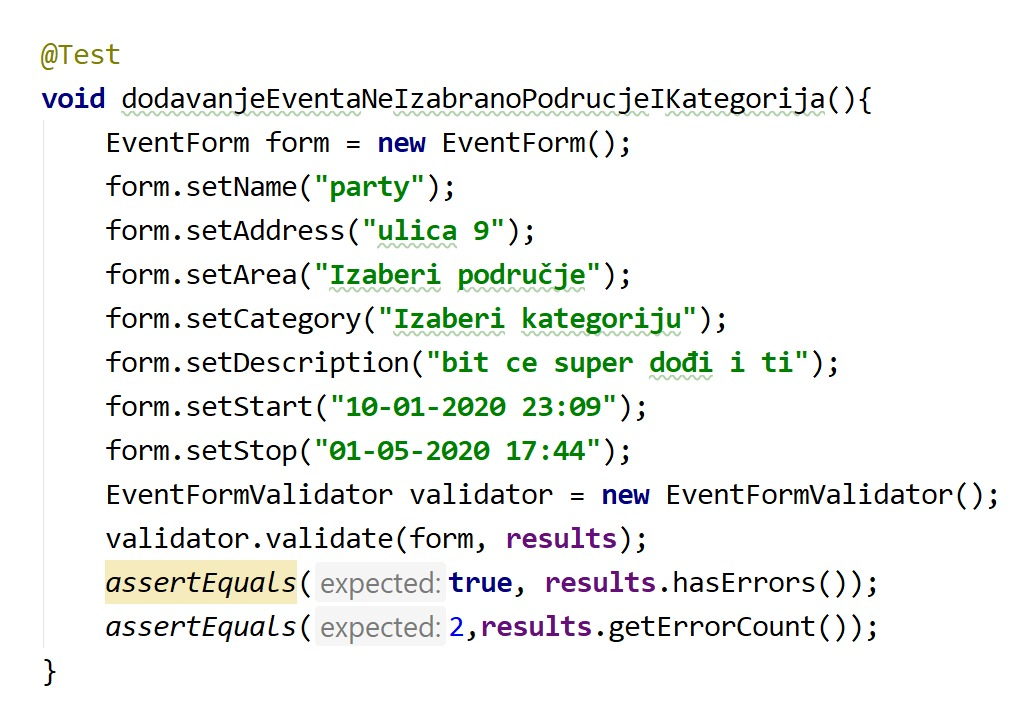
\includegraphics[scale=0.4]{slike/kategorija_i_mjesto_dogadaja.jpeg}
	\centering
	\caption{Ispitivanje kategorije i mjesta događaja}
	\label{fig:kategorijaimjestodogadaja}
\end{figure}

\normalfont Slika \ref{fig:rezultatitestiranja} pokazuje ispravni rezultat svih testova što znaći da je validator dobro implementiran.

\begin{figure}[H]
	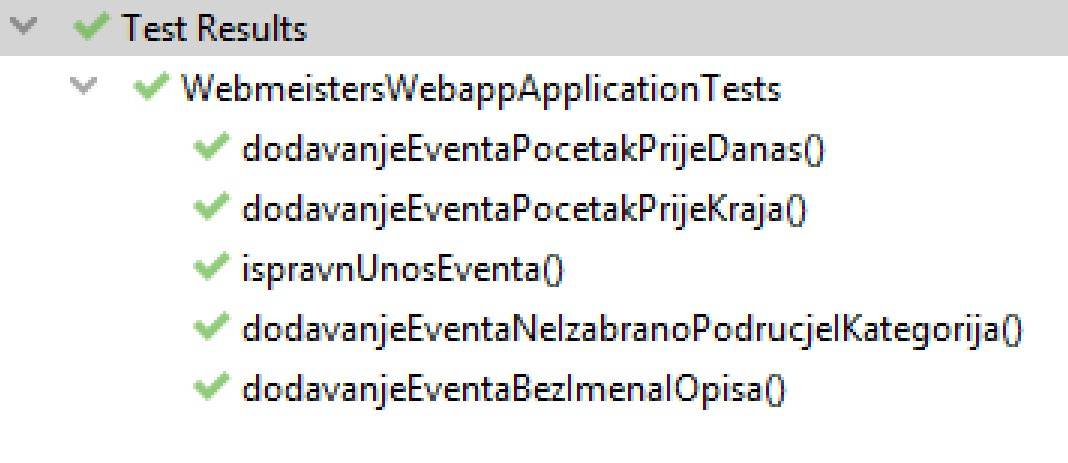
\includegraphics[scale=0.4]{slike/rezultati_testiranja.jpeg}
	\centering
	\caption{Rezultati testiranja}
	\label{fig:rezultatitestiranja}
\end{figure}

\bigskip

\subsection{Ispitivanje sustava}

\bigskip

\normalfont Svi testovi su izvršeni preko Seleniuma i testiraju se neke funkcionalosti organizatora.

\bigskip

\normalfont\noindent Na slici \ref{fig:addevent} nalazi se test dodavanja događaja kod organizatora. Također na slikama \ref{fig:addeventerrors} i \ref{fig:addeventwrong} testiraju se notifikacije tijekom izostajanja unosa podataka kod dodavanja događaja i krivim postavljanjem datuma.

\begin{figure}[H]
	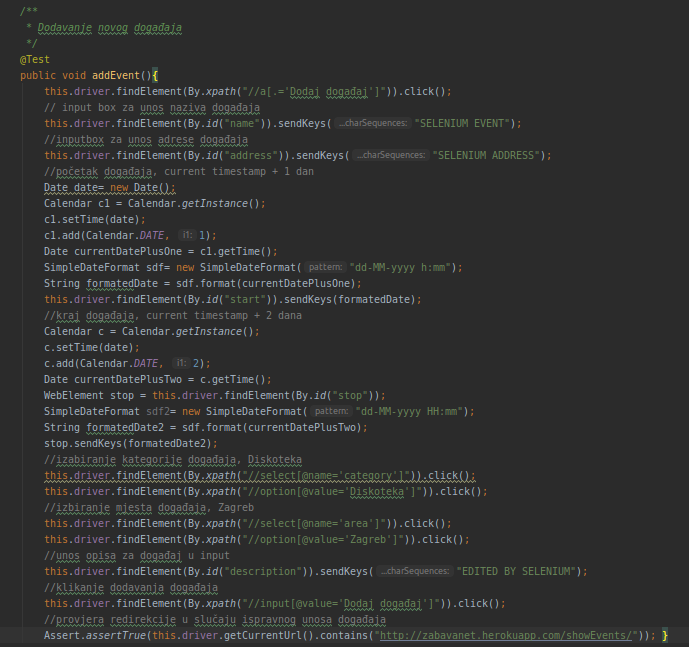
\includegraphics[scale=0.4]{slike/addEvent.PNG}
	\centering
	\caption{Dodavanje novog događaja}
	\label{fig:addevent}
\end{figure}

\begin{figure}[H]
	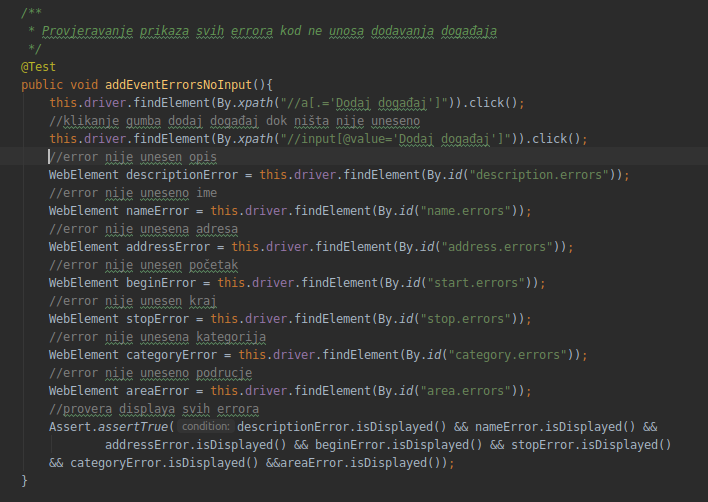
\includegraphics[scale=0.4]{slike/addEventErrorsNoInput.PNG}
	\centering
	\caption{Provjeravanje prikaza svih errora kod ne unosa dodavanja događja}
	\label{fig:addeventerrors}
\end{figure}

\begin{figure}[H]
	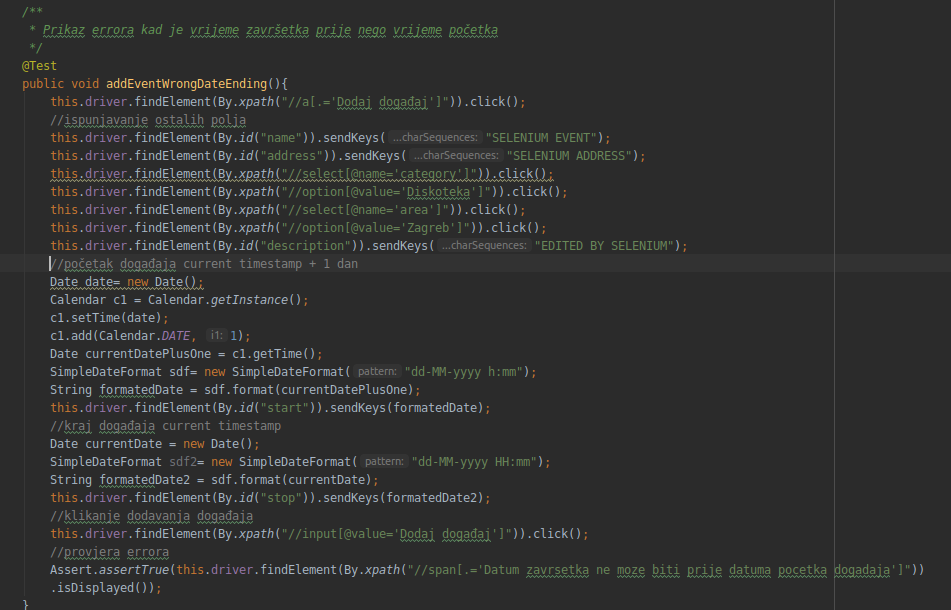
\includegraphics[scale=0.4]{slike/addEventWrongDateEnding.PNG}
	\centering
	\caption{Prikaz errora kada je vrijeme završetka prije noego vrijeme početka}
	\label{fig:addeventwrong}
\end{figure}


\normalfont\noindent Na slici \ref{fig:changename} testira se funkcionalost promjene imena organizatora.

\begin{figure}[H]
	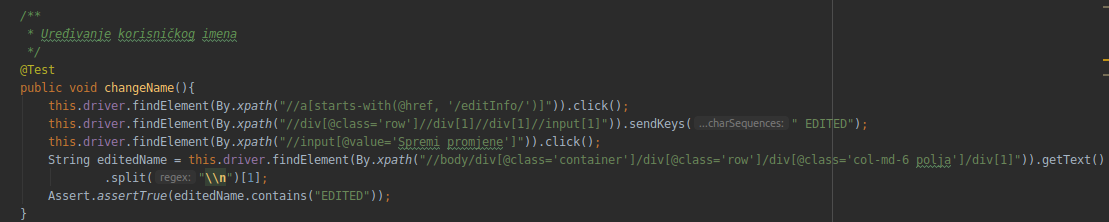
\includegraphics[scale=0.4]{slike/changeName.PNG}
	\centering
	\caption{Uređivanje korisničkog imena}
	\label{fig:changename}
\end{figure}

\normalfont\noindent Na slici \ref{fig:logmein} nalazi se metoda kojom se ulogirava u organizatorov račun, koja se poziva svaki put u metodi sa slike \ref{fig:loginvisitprofile} prije svakog testa.

\begin{figure}[H]
	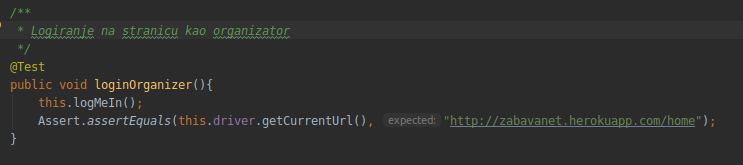
\includegraphics[scale=0.4]{slike/loginOrganizer.PNG}
	\centering
	\caption{Registracija kao organizator}
	\label{fig:loginOrganizer}
\end{figure}

\begin{figure}[H]
	\includegraphics[scale=0.4]{slike/LogMeIn.PNG}
	\centering
	\caption{Metoda pri registraciji}
	\label{fig:logmein}
\end{figure}

\begin{figure}[H]
	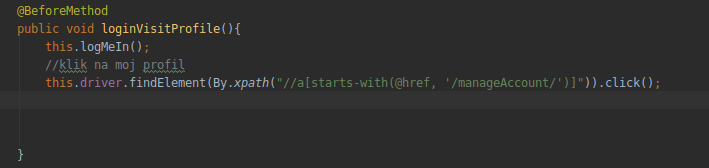
\includegraphics[scale=0.4]{slike/loginVisitProfile.PNG}
	\centering
	\caption{Registracija}
	\label{fig:loginvisitprofile}
\end{figure}

\normalfont\noindent Na slici \ref{fig:results} nalaze se rezultati testiranja.

\begin{figure}[H]
	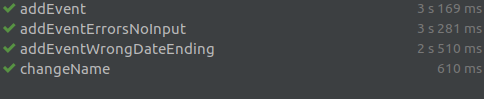
\includegraphics[scale=0.4]{slike/results.PNG}
	\centering
	\caption{Rezultati testiranja}
	\label{fig:results}
\end{figure}
\eject 


\section{Dijagram razmještaja}

\normalfont{Dijagram razmještaja prikazuje generalnu topologiju sustava koji se koristi
	kako bi resursi bili optimalno raspoređeni. Predstavlja statički pogled na razmještaj
	sklopovskih i programskih komponenata.}

\normalfont\noindent{Na poslužiteljskom
	računalu se nalaze web poslužitelj i poslužitelj baze podataka. Klijenti koriste web
	preglednik kako bi pristupili web aplikaciji te se komunikacija između računala korisnika i poslužitelja odvija preko HTTP veze.}

\begin{figure}[H]
	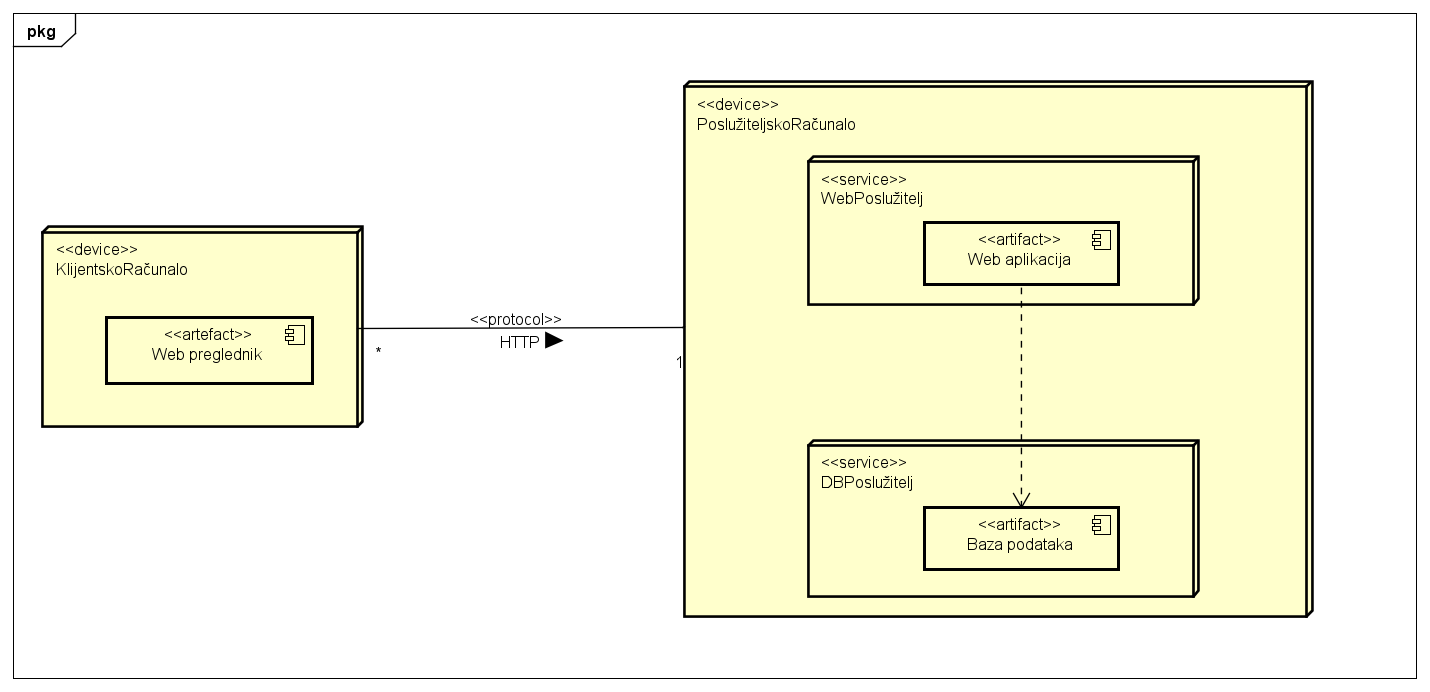
\includegraphics[scale=0.4]{slike/DijagramRazmjestaja.PNG}
	\centering
	\caption{Dijagram razmještaja}
	\label{fig:promjene}
\end{figure}

\eject 

\section{Upute za puštanje u pogon}

\normalfont Kako bi pustili aplikaciju u pogon, potrebno je napraviti deploy. U našem slučaju taj deploy smo napravili na Heroku. 

\normalfont\noindent Kako bi napravili deploy aplikacije na Heroku potrebno je napraviti korisnički račun.

\begin{figure}[H]
	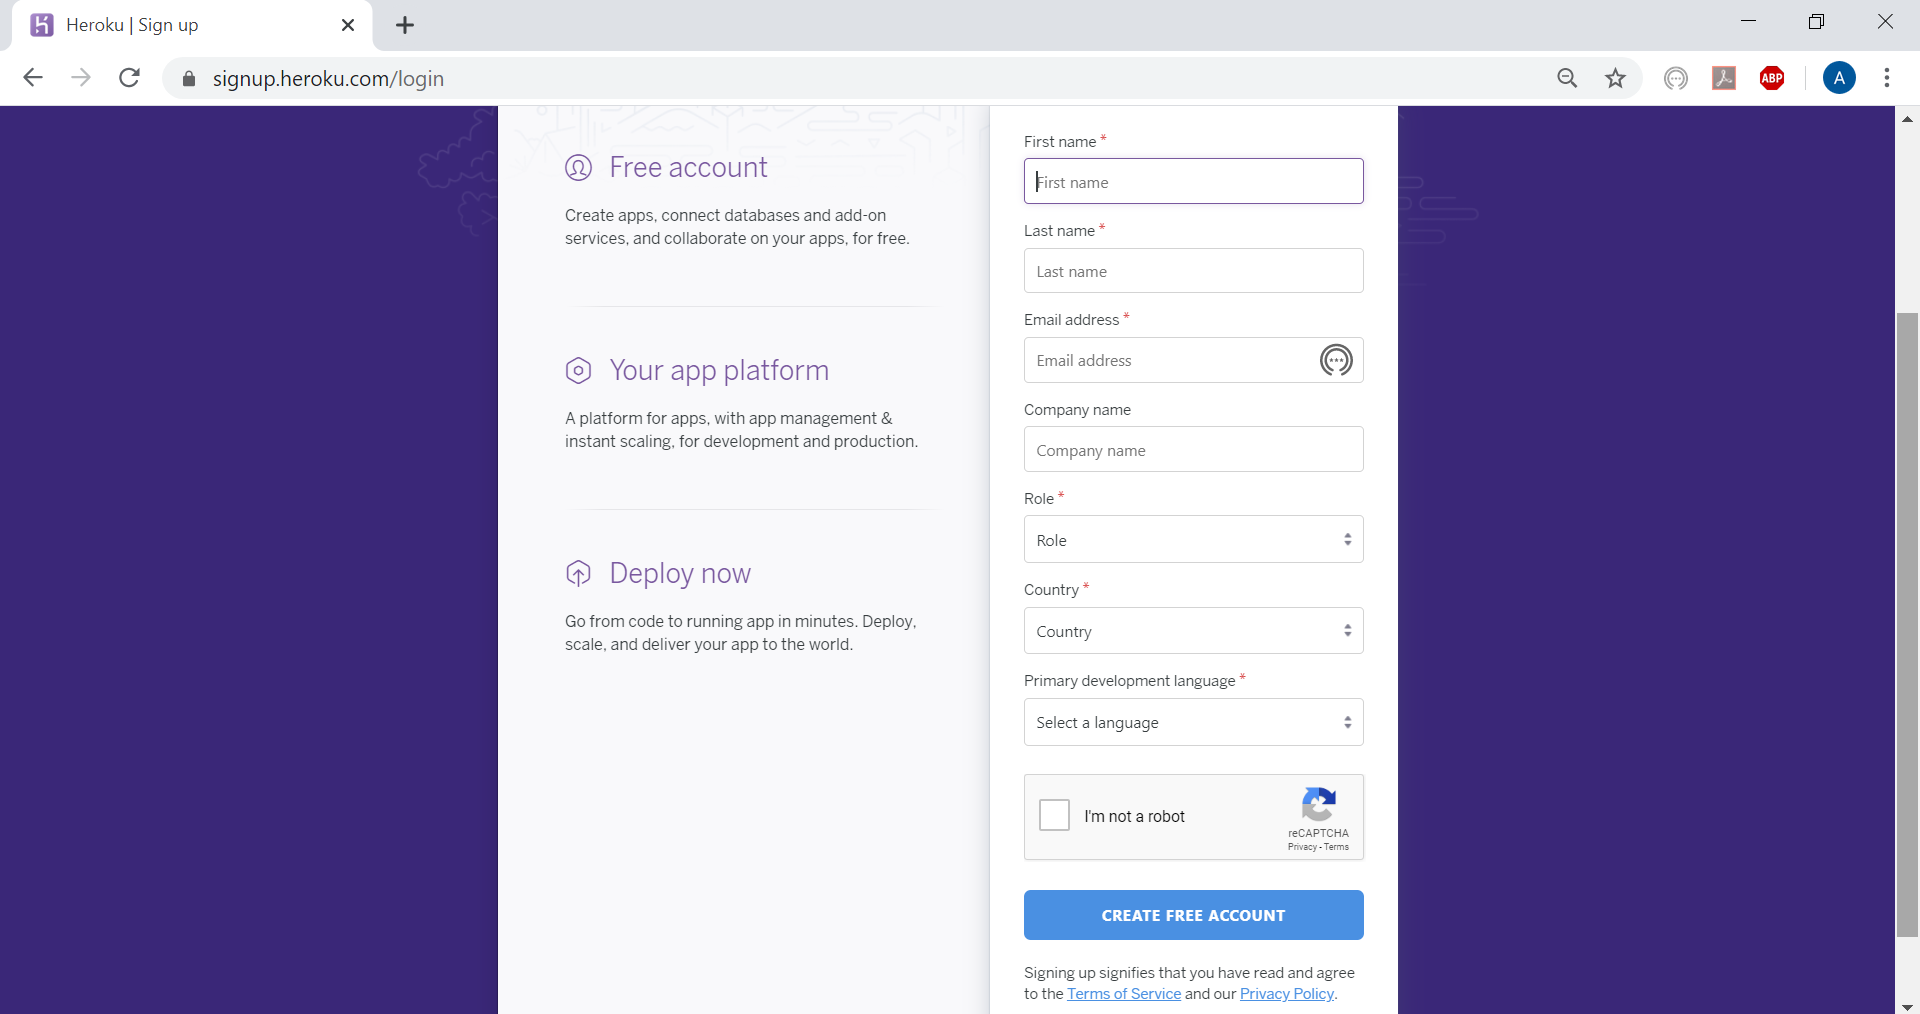
\includegraphics[scale=0.4]{slike/korisnicki_racun.PNG}
	\centering
	\caption{Izrada korisničkog računa}
	\label{fig:pogon1}
\end{figure}

\normalfont Nakon što se napravi korisnički račun koji je besplatan, na mail adresu koja je upisana dobije se link na koji se mora kliknuti kako bi se potvrdio račun i postavila lozinka.

\begin{figure}[H]
	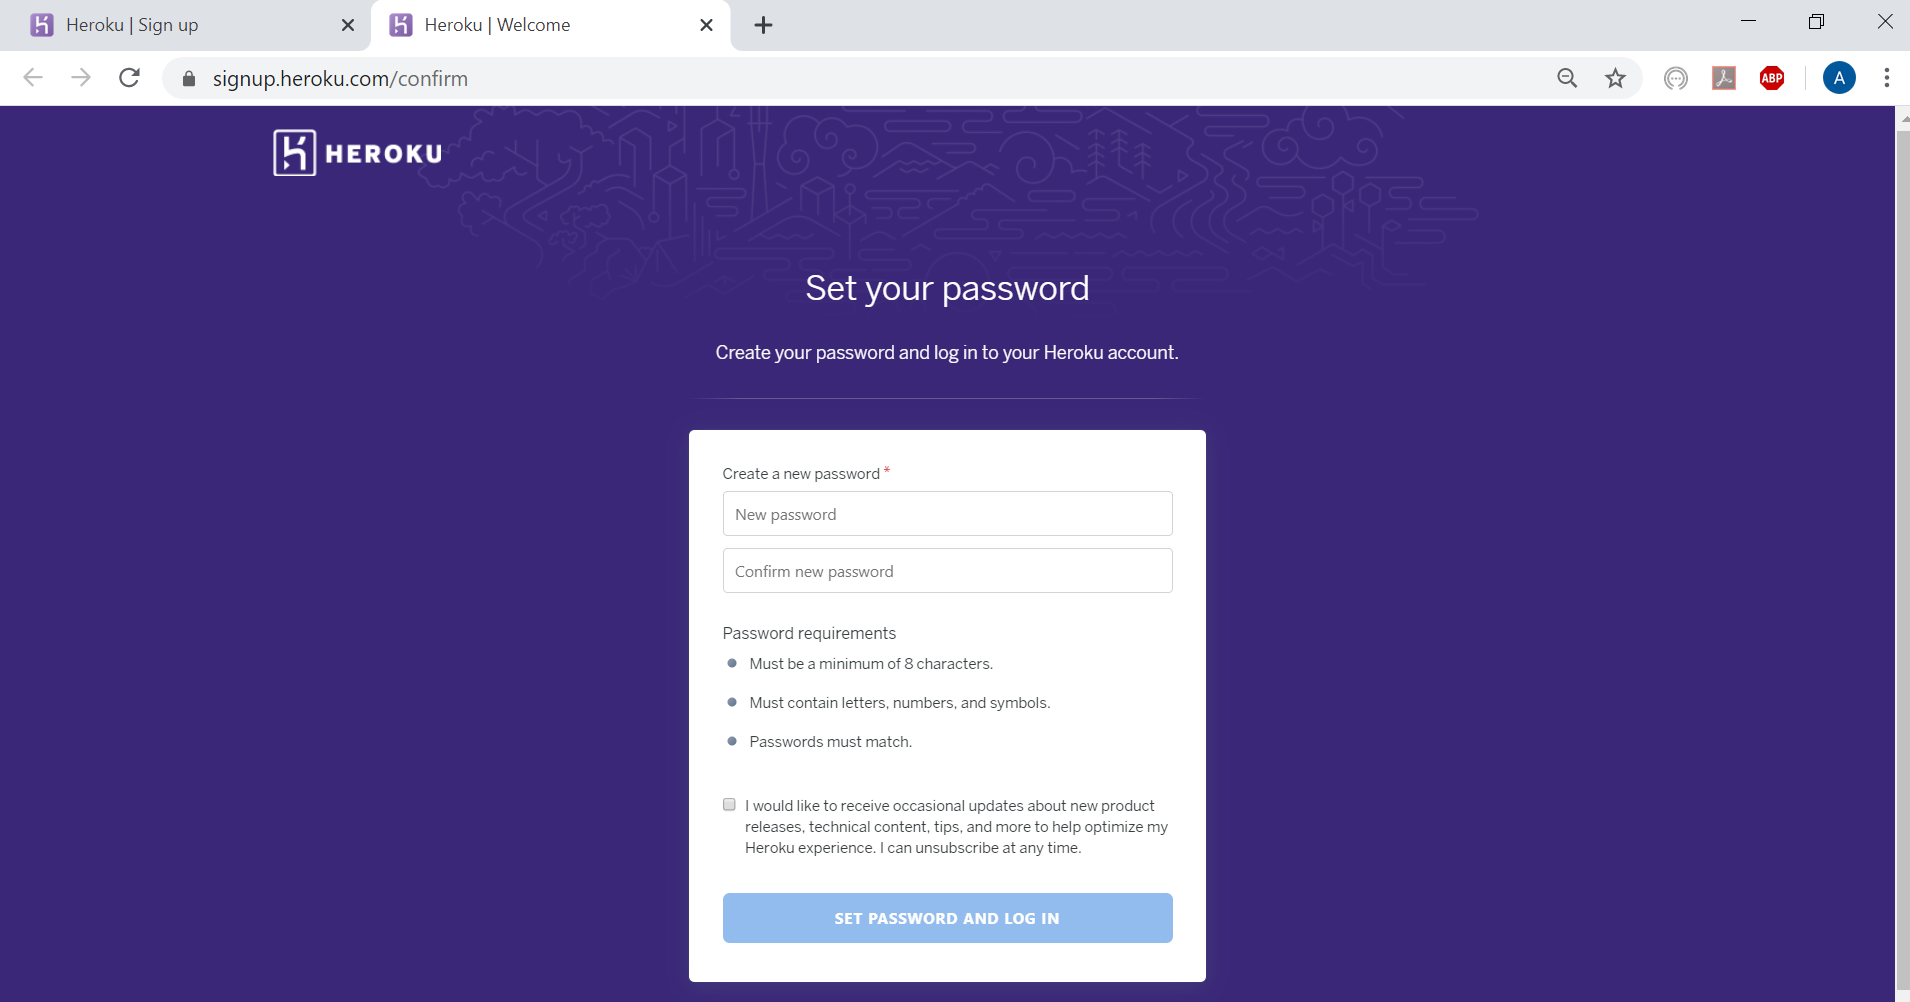
\includegraphics[scale=0.4]{slike/potvrda_lozinke.PNG}
	\centering
	\caption{Potvrda lozinke}
	\label{fig:pogon2}
\end{figure}

\normalfont Nakon što se postavi lozinka, moguće je dodati aplikaciju.

\begin{figure}[H]
	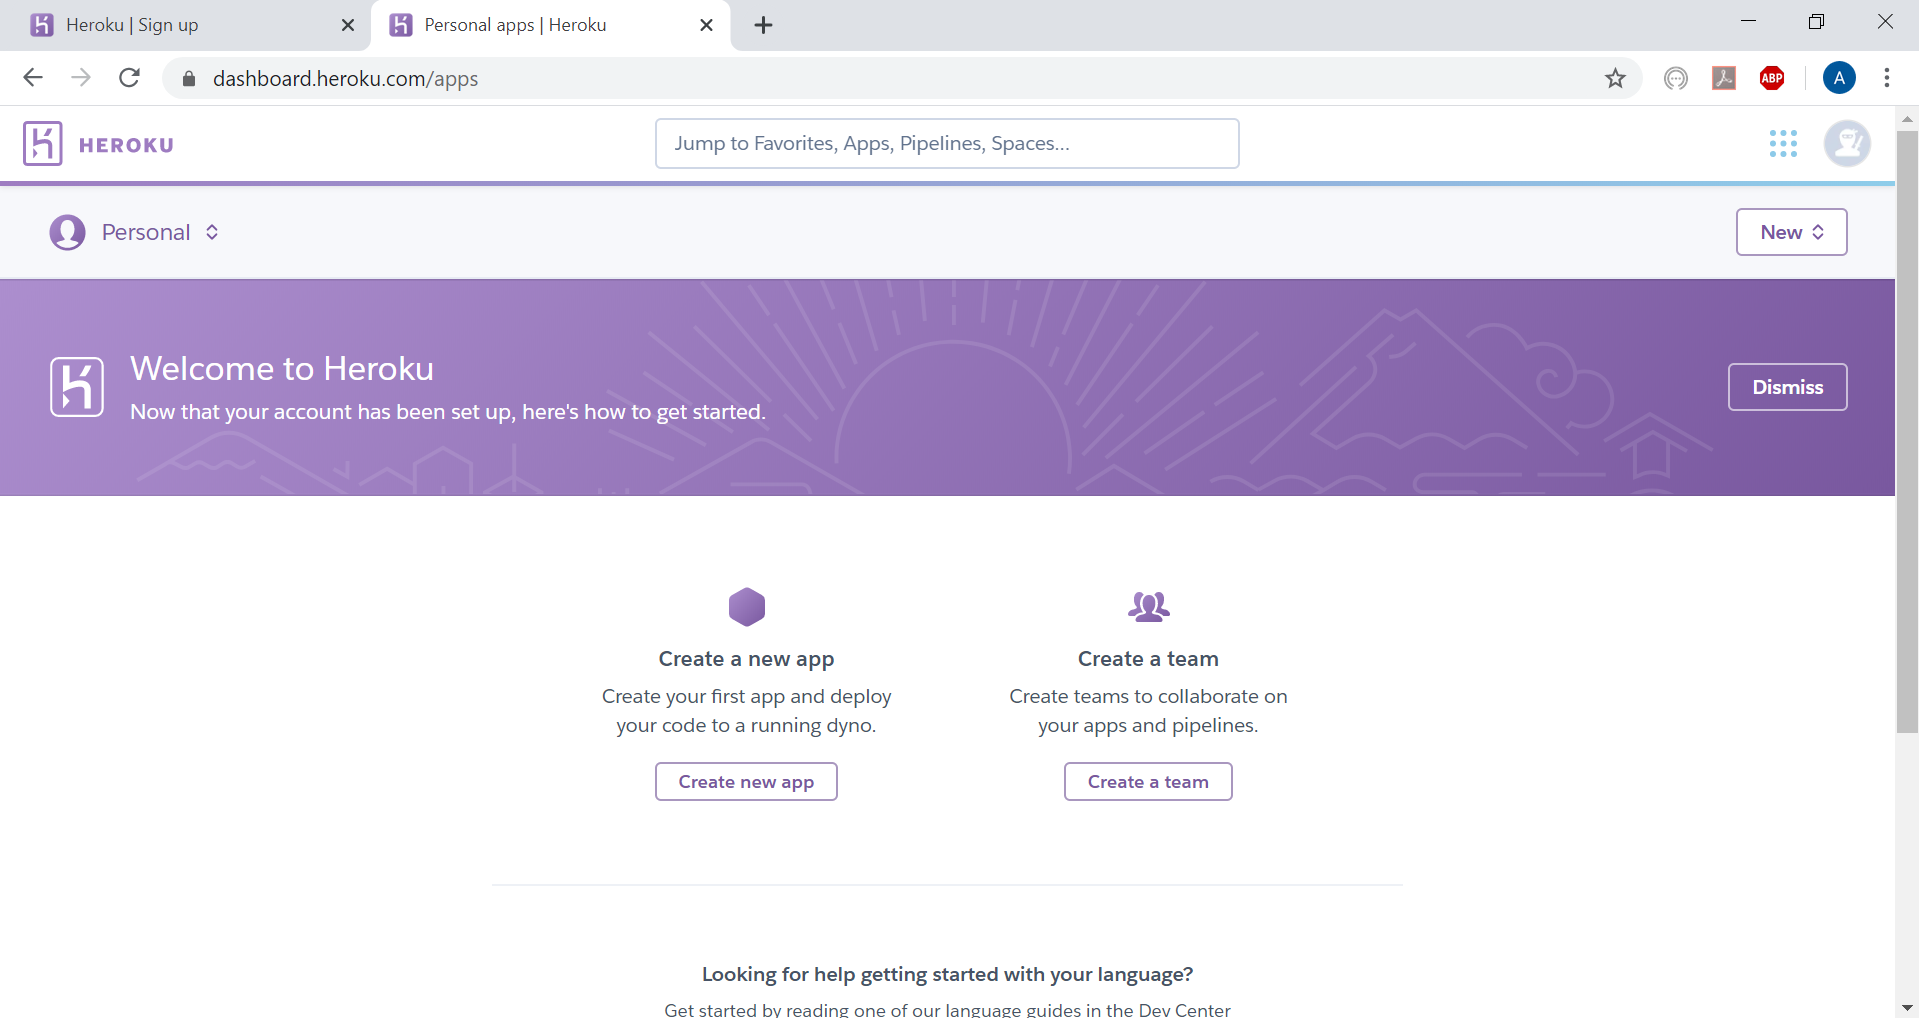
\includegraphics[scale=0.4]{slike/dodavanje_aplikacije.PNG}
	\centering
	\caption{Dodavanje aplikacije}
	\label{fig:pogon3}
\end{figure}

\normalfont Tu se odabere opcija „Create a new app“ te se nakon toga odabere ime aplikacije i regija.

\normalfont Mi smo odabrali zabavanet2 i „Europe“

\begin{figure}[H]
	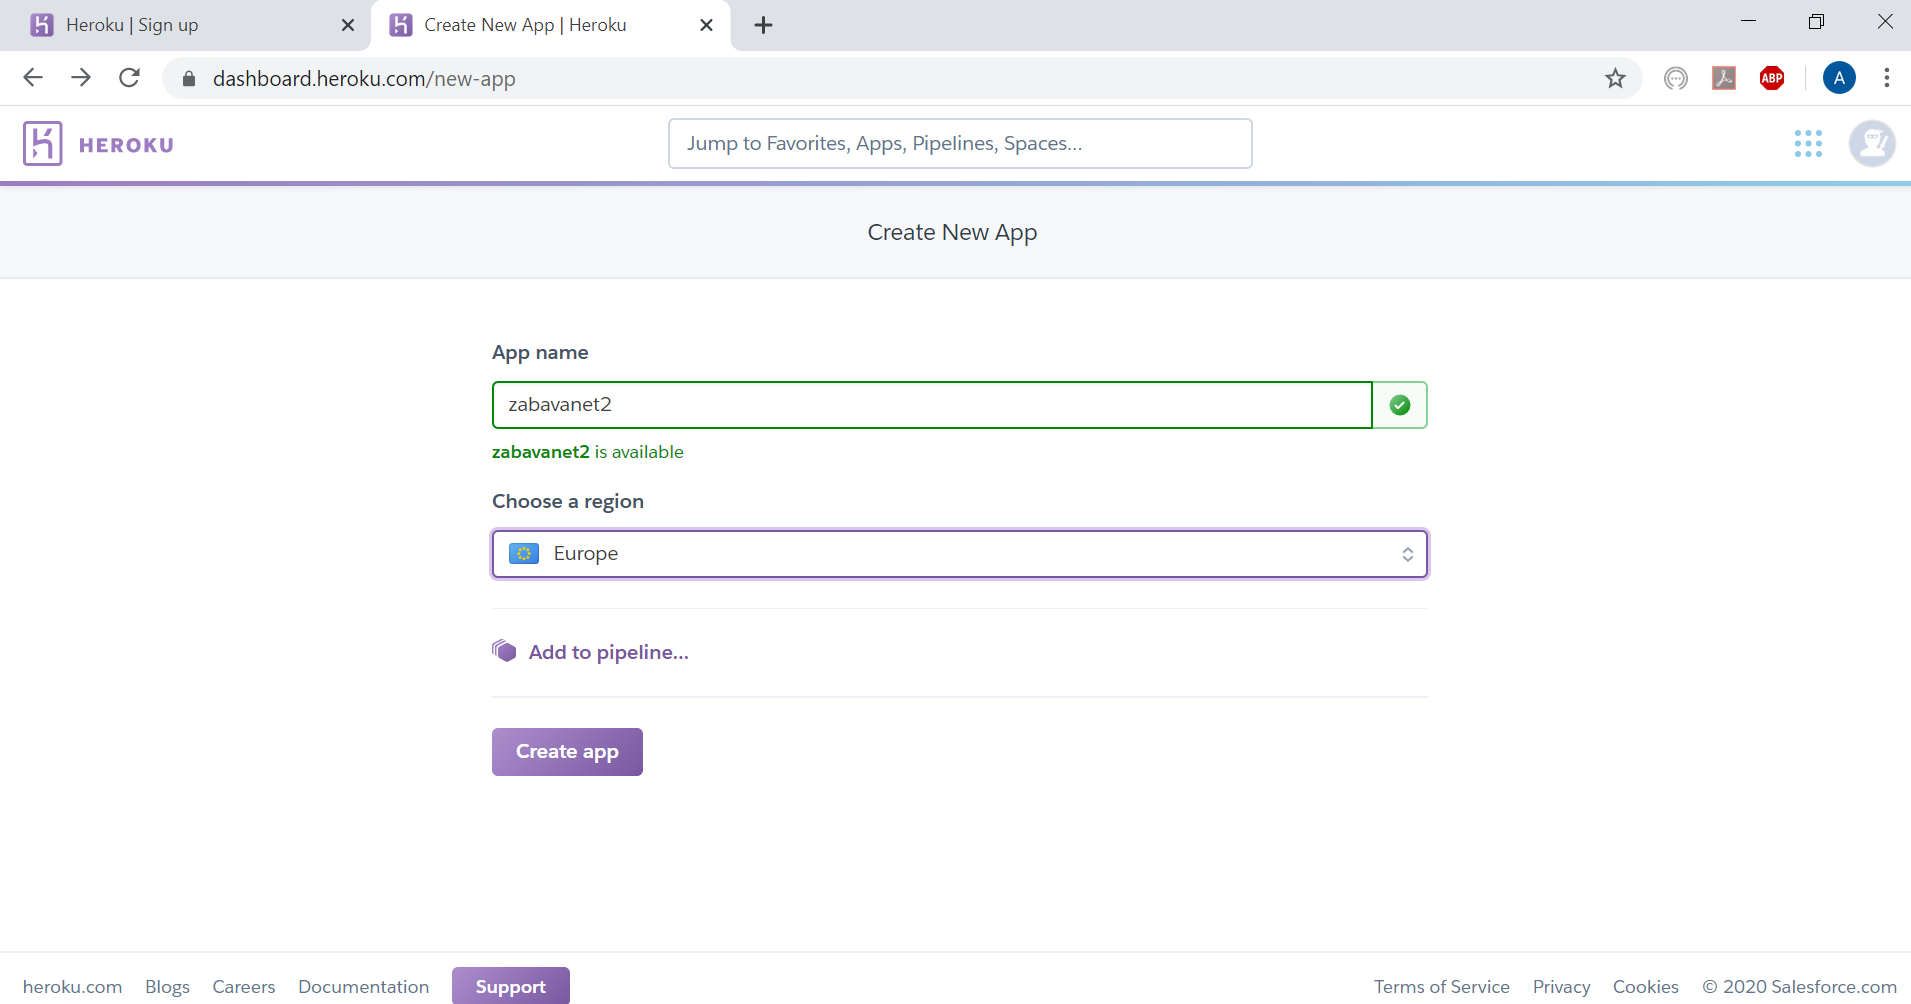
\includegraphics[scale=0.4]{slike/ime_i_regija.PNG}
	\centering
	\caption{Odabir imena i regije}
	\label{fig:pogon4}
\end{figure}

\normalfont Dalje sve što treba napraviti je slijediti ove upute i aplikacija je postavljena. 

\begin{figure}[H]
	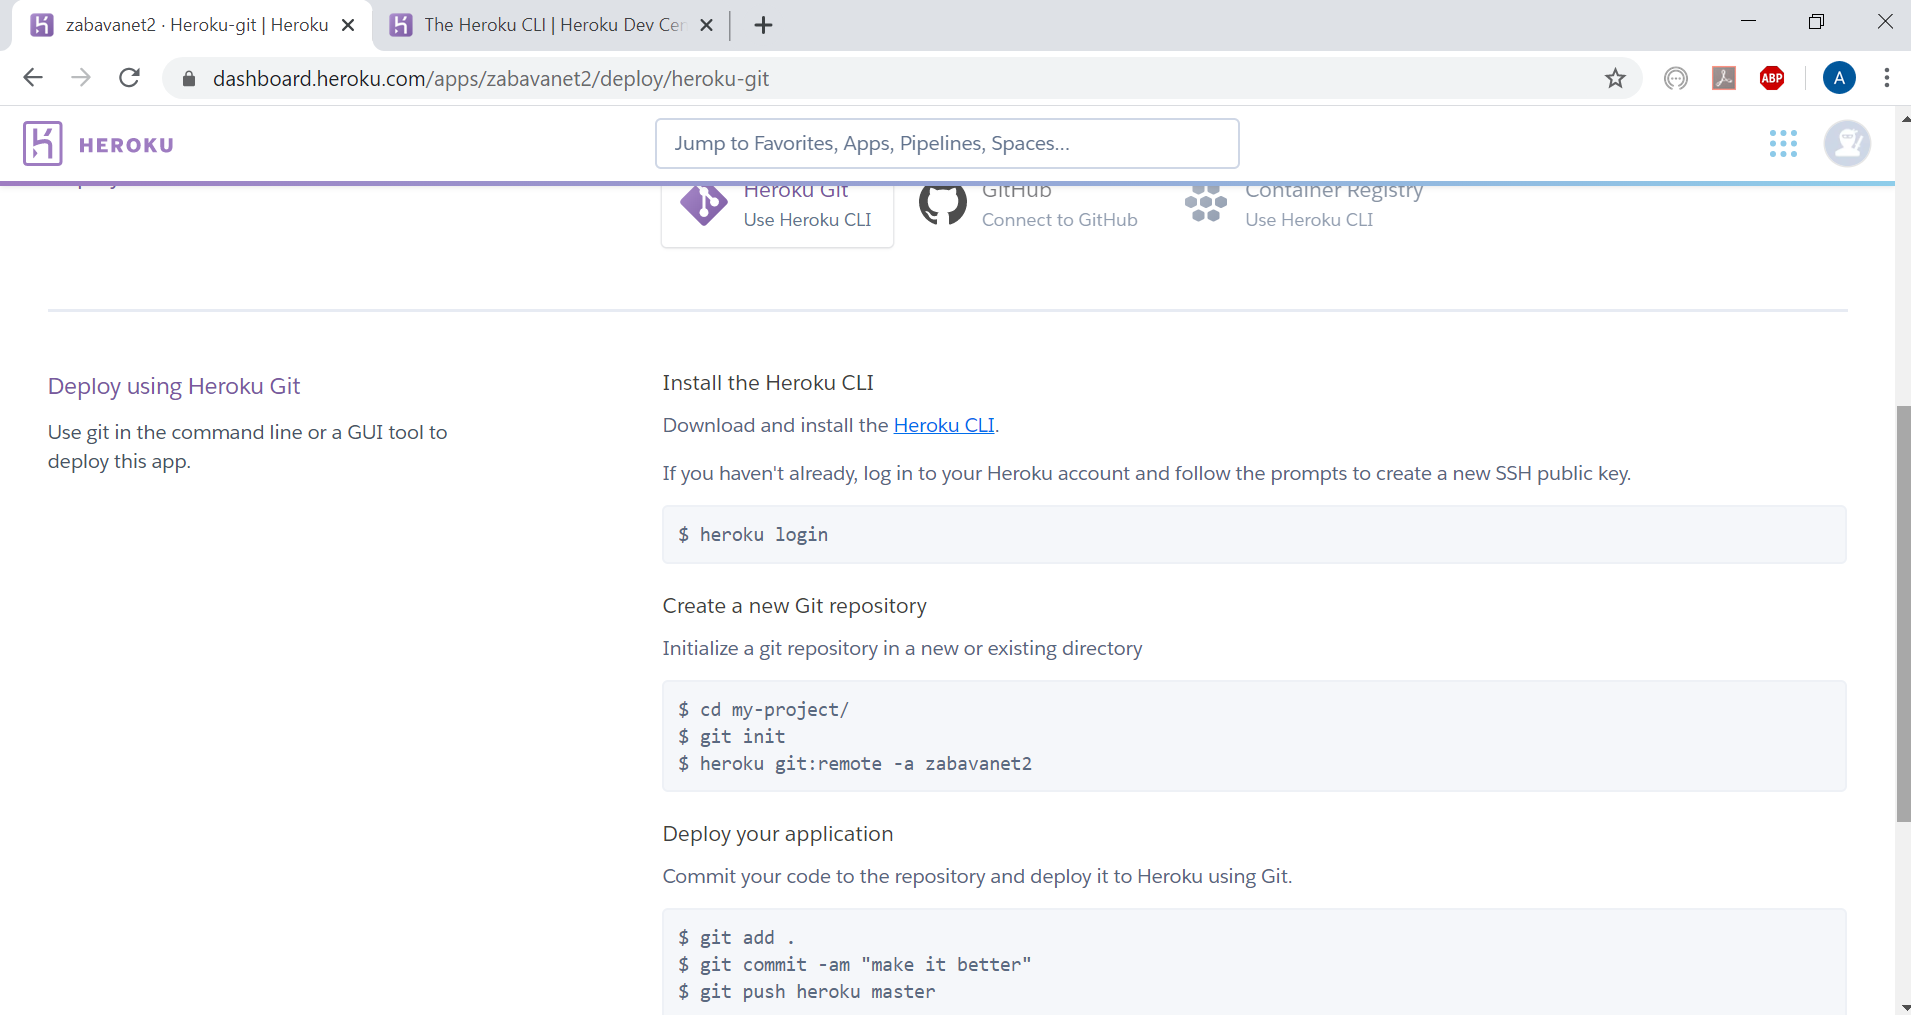
\includegraphics[scale=0.4]{slike/upute.PNG}
	\centering
	\caption{Instalacija}
	\label{fig:pogon5}
\end{figure}

\noindent1. Treba instalirati Heroku CLI, link je u uputam Herokua.\\
2. Napravimo vlastitu mapu na računalu „herokuDeploy2“ u koju se kopira sav potreban sadržaj aplikacije.\\
3.Nakon što je to učinjeno, u Command promptu na Windowsima možemo izvršiti ove naredbe.\\
4. Aplikacija bi ukoliko ne bude nikakvih problema trebala biti deployjana i dobit ćemo ovakvu poruku : „Build success“.\\
To bi značilo da je sve uspješno napravljeno i možemo pristupiti aplikaciji na dobivenom linku.
\eject 